%-------------------------------------------------------------------------------
% LATEX TEMPLATE ARTIKEL
%-------------------------------------------------------------------------------
% Dit template is voor gebruik door studenten van de de bacheloropleiding 
% Informatica van de Universiteit van Amsterdam.
% Voor informatie over schrijfvaardigheden, zie 
%                               https://practicumav.nl/schrijven/index.html
%
%-------------------------------------------------------------------------------
%	PACKAGES EN DOCUMENT CONFIGURATIE
%-------------------------------------------------------------------------------

\documentclass{uva-inf-article}
\usepackage[english]{babel}
\usepackage{tikz}
\usepackage{pdflscape}
\usepackage{todonotes}
\usepackage{subfig}

\usepackage[style=authoryear-comp]{biblatex}
\addbibresource{references.bib}

%-------------------------------------------------------------------------------
%	GEGEVENS VOOR IN DE TITEL, HEADER EN FOOTER
%-------------------------------------------------------------------------------

% Geef je artikel een logische titel die de inhoud dekt.
\title{Bones and Joints}

% Vul de naam van de opdracht in zoals gegeven door de docent en het type 
% opdracht, bijvoorbeeld 'technisch rapport' of 'essay'.
% \assignment{}
% \assignmenttype{}

% Vul de volledige namen van alle auteurs in en de corresponderende UvAnetID's.
\authors{Jari Andersen}
% \uvanetids{}

% Vul de naam van je tutor, begeleider (mentor), of docent / vakcoördinator in.
% Vermeld in ieder geval de naam van diegene die het artikel nakijkt!
% \tutor{}
% \mentor{}
% \docent{}

% Vul hier de naam van je tutorgroep, werkgroep, of practicumgroep in.
% \group{SignLab, VisualisationLab}

% Vul de naam van de cursus in en de cursuscode, te vinden op o.a. DataNose.
% \course{}
% \courseid{}

% Dit is de datum die op het document komt te staan. Standaard is dat vandaag.
\date{\today}

%-------------------------------------------------------------------------------
%	VOORPAGINA 
%-------------------------------------------------------------------------------

\begin{document}
\maketitle
% \tableofcontents
% \newpage
%-------------------------------------------------------------------------------
%	INHOUDSOPGAVE EN ABSTRACT
%-------------------------------------------------------------------------------
% Niet toevoegen bij een kort artikel, zeg minder dan 10 pagina's!

%TC:ignore
%\tableofcontents
%\begin{abstract}
%\end{abstract}
%TC:endignore

%-------------------------------------------------------------------------------
%	INHOUD
%-------------------------------------------------------------------------------
% Hanteer bij benadering IMRAD: Introduction, Method, Results, Discussion.
\section{Introduction}
In avatar skeletons, we often refer to skeletal "bones," which is quite misleading. Animation and skeletal mesh files are actually built from joints, not bones. Additionally, it's a common misconception that each joint can only rotate, leading to most motions through different rotations in a hierarchy. This isn't accurate. Joints can both rotate and translate. In this report, I will do my best to clear up any misconceptions.

\subsection{Avatar skeletons and animations}
Avatar skeletons form the fundamental framework upon which animated characters are built in digital environments. At their core, these skeletons consist of interconnected joints that define the character's movement capabilities. Weights play a crucial role in determining how the movement of joints influences the deformation of the mesh. These weights, often referred to as weight painting\footnote{\url{https://docs.blender.org/manual/en/latest/sculpt_paint/weight_paint/introduction.html}}, are assigned to vertices of the mesh to control the extent to which each joint affects them.

Each vertex on the mesh is typically influenced by multiple joints, with specific weights assigned to each joint's influence. For example, consider the arm of an animated character. Vertices near the elbow joint would have higher weights associated with the elbow joint, allowing them to move more when the elbow bends. Conversely, vertices closer to the shoulder would have higher weights for the shoulder joint, enabling the upper arm to move appropriately when the shoulder rotates.

By combining joints and weights, animators can bring an avatar to life by changing the joint orientation and translation (if needed) over time.



\subsection{Complex handforms}
Complex skeletons contain a greater number of joints, allowing for more detailed and precise animations. Conversely, less complex skeletons have fewer joints, which can simplify the animation process but at the cost of reducing the range and subtlety of movements.

A prime example of this difference is found in the hands. A complex hand skeleton might include joints for each phalange (finger bone), including the metacarpals, which are the bones in the hand that connect the fingers to the wrist. The metacarpals allow for intricate hand movements such as creating a cupping handform. In contrast, a less complex hand skeleton might omit the metacarpals limiting the hand's movement capabilities. Without these joints, certain movements become impossible or less convincing. For example, creating a natural-looking cupping handform relies on the ability to move not just the fingers but also the metacarpals. Without these joints, the hand might appear stiff or unrealistic when attempting complex gestures. Figure \ref{fig:ssrpm} compares the stretchsense/metahuman hands with the ReadyPlayerMe hands. The green dots are the joints. In figure \ref{fig:rpmvsmeta} the same comparison can be viewed in Unreal Engine.

\subsubsection{Effects on retargeting}
Retargeting is the process of transferring animations from one skeleton to another. When retargeting animations from a complex skeleton to a less complex one, there can be significant losses in movement fidelity. This is particularly evident in the hands.

For example, if an animation designed for a hand with complete joint articulation (including the metacarpals) is retargeted to a hand skeleton with only the basic finger joints, the resulting animation will lack the subtle movements of the original. Specifically, movements such as cupping the hand or other complex gestures that require metacarpal involvement will be compromised.

In our pipeline, we have retargeted animations recorded in the StretchSense HandEngine software and remapped these to a ReadyPlayerMe avatar. Besides not being able to do cupping motions, we have also run into other strange behaviour of the ReadyPlayerMe hands. For example, the thumb1 joint has the tendency to be rotated by 90 degrees depending on the calibration in HandEngine. This can be solved by using more calibrations related to the thumb, but it is interesting to see how the animations on the HandEngine hand doesn't match the animations on the ReadyPlayerMe hand.


\begin{figure}[hbt!]
    \centering
    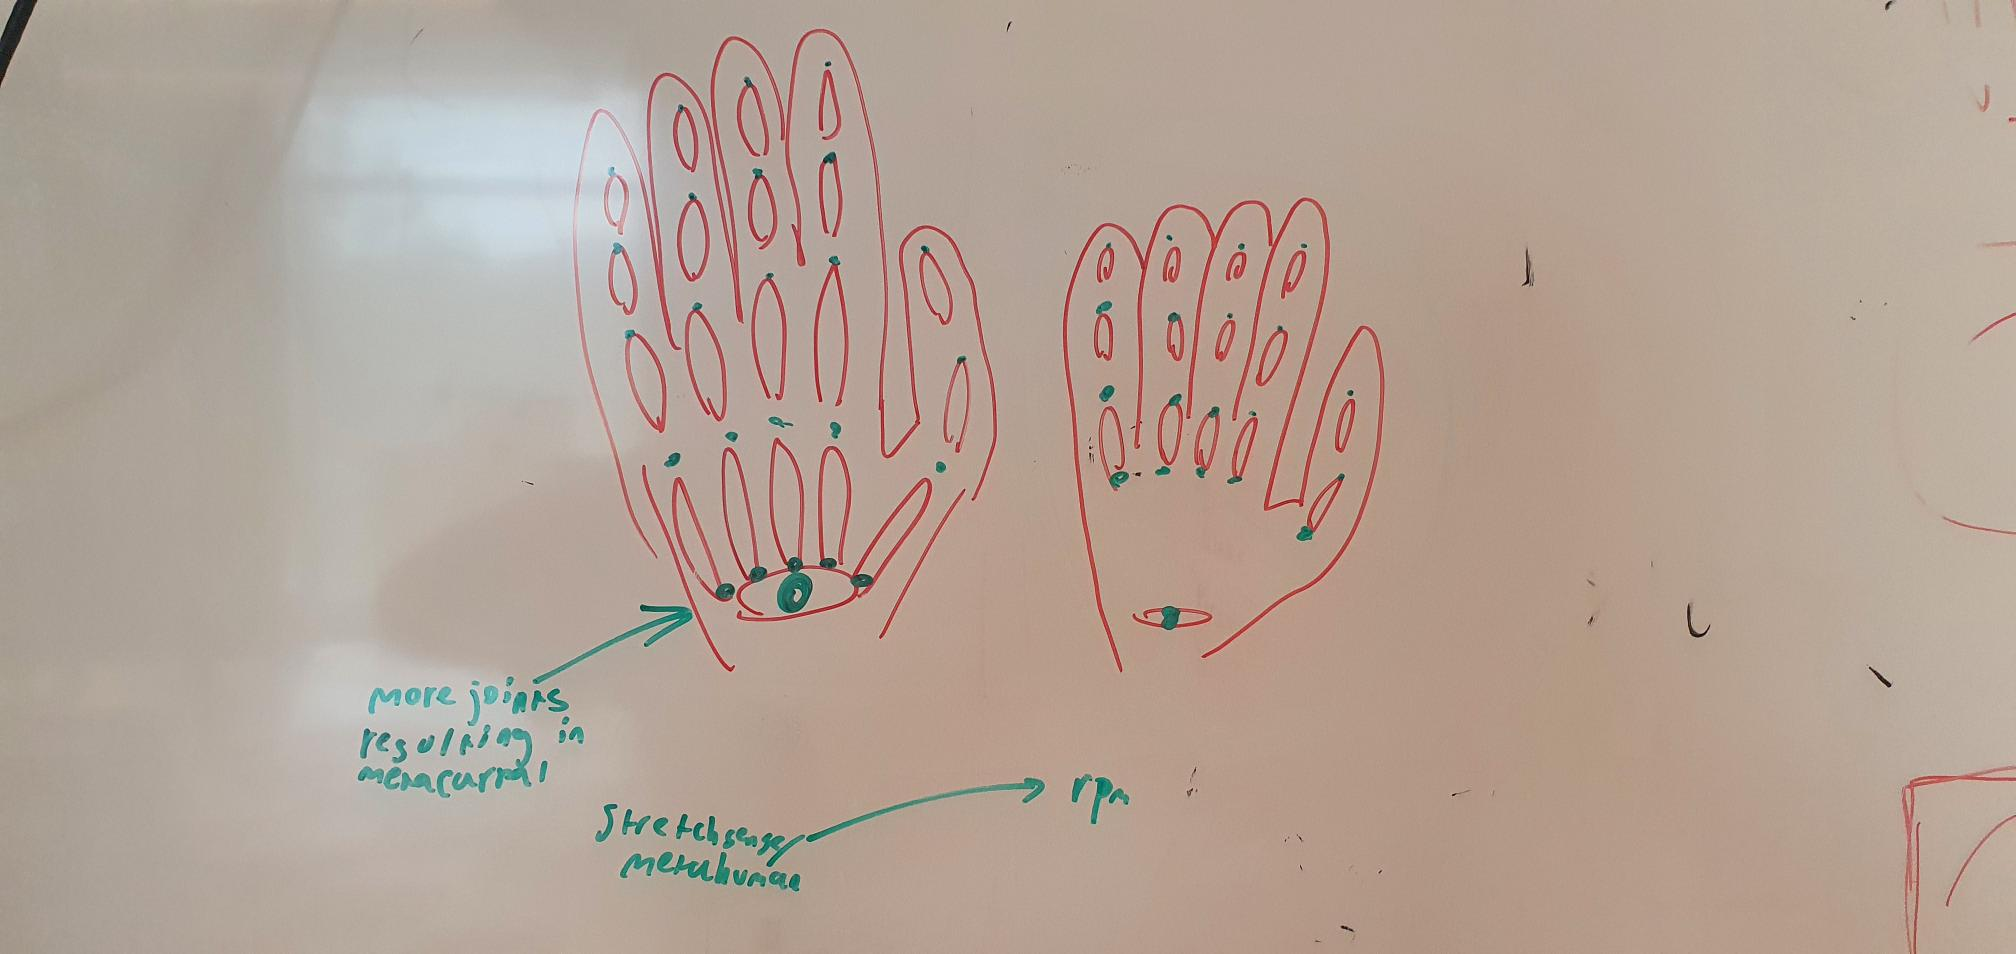
\includegraphics[width=0.8\textwidth]{imgs/complexHandNonComplexHand.jpg}
    \caption{Comparison of stretchsense/metahuman with RPM hand}
    \label{fig:ssrpm}
\end{figure}

\subsection{Why Translation is Important in Skeletal Animations}
Translation in skeletal animations is crucial for several reasons:

\begin{itemize}
    \item \textbf{Versatility Across Different Mesh Types:}\\
Skeletal animation is not limited to humanoid avatars. It can be applied to various meshes, including animals, mythical creatures, and even inanimate objects that require deformation. Translation allows animators to position joints in ways that achieve the desired effect, making the technique adaptable to a broad range of animation scenarios.

    \item \textbf{Enhanced Expressiveness:}\\
Translation enables more dynamic and exaggerated movements, essential for certain styles of animation, especially in cartoons. The ability to stretch and squash joints adds a layer of expressiveness that pure rotation cannot achieve. This helps in creating characters that are more lively and engaging.

    \item \textbf{Detailed Deformations:}\\
In realistic animations, especially those using motion capture, translation can mimic subtle deformations of the body, such as the stretching and compressing of skin and muscles. This adds a level of realism and nuance to the animation, making movements more believable. High-quality motion capture systems may capture these details, and translating joints helps replicate these effects in the final animation.

    \item \textbf{Compensating for Missing Joints:}\\
While translation cannot fully replace the functionality of missing joints, it can help in approximating certain movements. For instance, in avatars with simplified skeletons, translation can be used to simulate some aspects of complex movements. However, for intricate actions like hand cupping, the presence of all relevant joints (like metacarpals) is essential for accurate reproduction. I have tried to mimic the cupping form by translating the joints in figure \ref{fig:cuppedNonCupped}. Although I got closer with translation then only rotation, we can still see that the palm is rigid.
\end{itemize}

In conclusion, translation is a vital component of skeletal animation, providing versatility, enhancing expressiveness, and enabling detailed deformations. It complements rotation to create more dynamic and lifelike animations, making it an indispensable tool for animators.

\begin{figure}[hbt!]
    \centering
    \subfloat[\centering ReadyPlayerMe hand joints]{{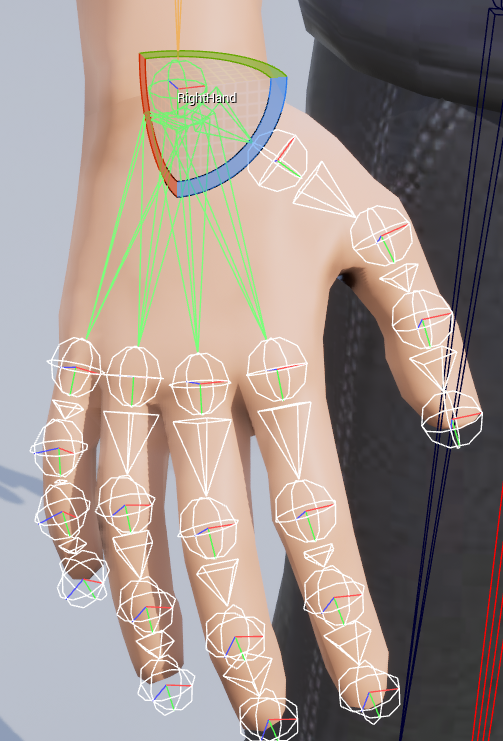
\includegraphics[height=6cm]{imgs/handBone.png} }}%
    \qquad
    \subfloat[\centering Metahuman hand joints]{{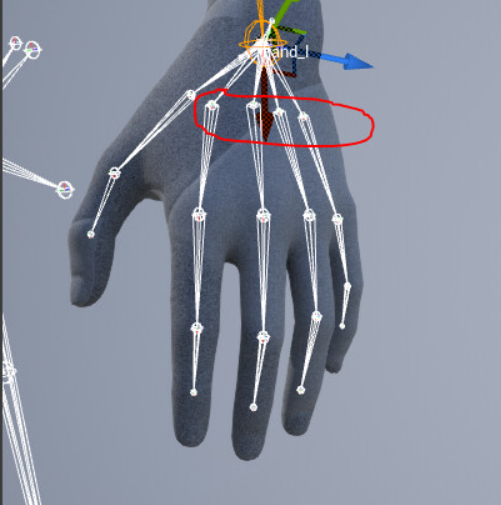
\includegraphics[height=6cm]{imgs/metahumanhand.png} }}%
    \caption{Comparison between ReadyPlayerMe and Metahuman hand joints. RPM misses metacarpals.}%
    \label{fig:rpmvsmeta}%
\end{figure}

\begin{figure}[hbt!]
    \centering
    \subfloat[\centering Not cupped hand]{{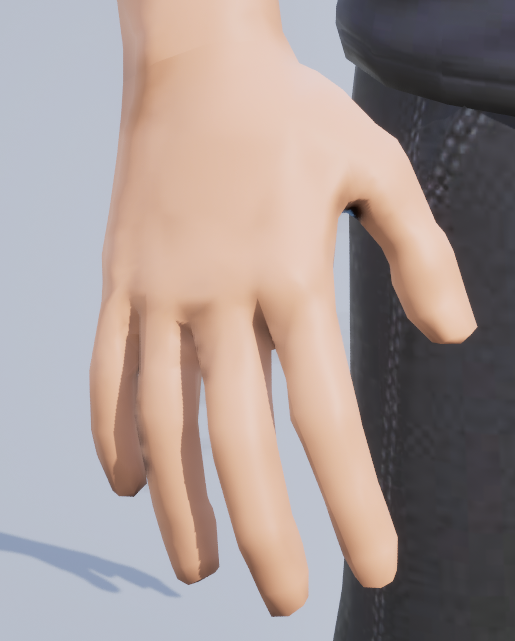
\includegraphics[width=5cm]{imgs/NotCupped.png} }}%
    \qquad
    \subfloat[\centering Cupped hand using only translation]{{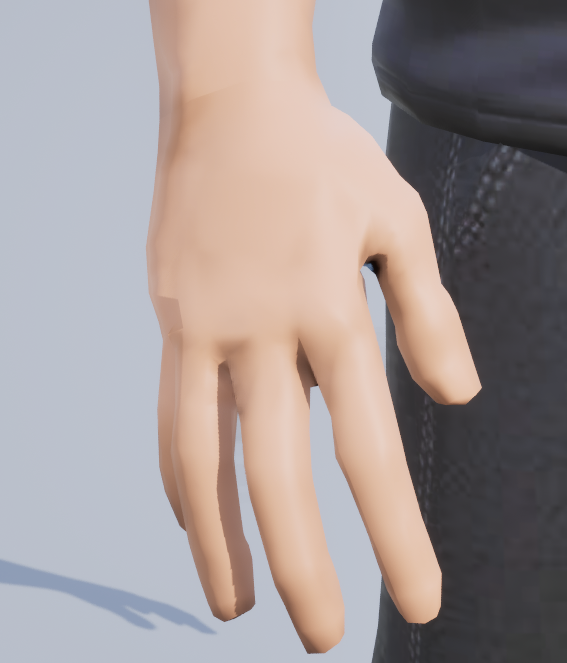
\includegraphics[width=5cm]{imgs/Cupped.png} }}%
    \caption{Comparison between a neutral hand, and a cupped hand using only translations on the joints}%
    \label{fig:cuppedNonCupped}%
\end{figure}
%-------------------------------------------------------------------------------
%	REFERENTIES
%-------------------------------------------------------------------------------

\printbibliography

%-------------------------------------------------------------------------------
%	BIJLAGEN 
%-------------------------------------------------------------------------------

%TC:ignore
% \appendix 
% \section{Bijlage {\LaTeX} code}
% Bijgevoegd zijn de \textattachfile{main.tex}{code} en 
% \textattachfile{references.bib}{bibliografie}.
%TC:endignore

%-------------------------------------------------------------------------------
\end{document}